\hthree{Allgemein}

\begin{figure}[H]
    \centering
    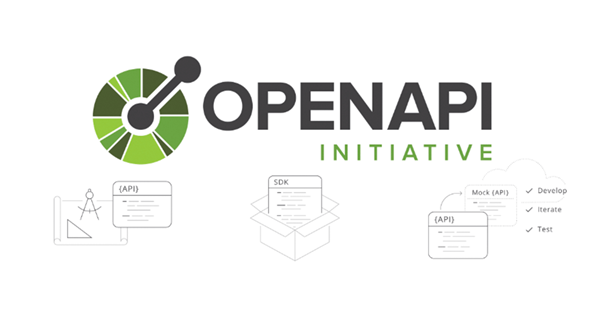
\includegraphics{media/OpenAPI/OpenAPILogo.png}
    \caption{OpenAPI-Logo \cite{RestSoap}}
\end{figure}

Die OpenAPI-Spezifikation ermöglicht es die Struktur einer REST-API so darzustellen, dass sie sowohl von Menschen als auch von Computern gelesen werden kann. Angefangen hat die OpenAPI-Spezifikation als Teil des Softwareprojekt "Swagger", einem Open-Source-Framework für HTTP-Webservices. Seit 2016 ist OpenAPI ein selbstständiges Projekt und wird von der OpenAPI-Initiative verwaltet. OpenAPI-Definitionen werden in einem Dokument abgespeichert. Geschrieben werden diese Dokumentationen dann entweder in JSON oder in YAML. Die Zelia-API wurde ebenfalls mithilfe von OpenAPI in YAML beschrieben. Wie ein OpenAPI-Dokument strukturiert ist, wird anhand der Zelia-API erläutert. Wichtig zu beachten ist bei der Verwendung von YAML die Einrückungen, die in dieser Sprache essenziell sind. \cite{OpenAPIGeneral}